\chapter{Draft: Cryptographic Primitives}

\section{Hash Functions}
\quad We use hash functions to represent objects in the network. A hash function is a mathematical function that takes in an arbitrary string input and outputs a unique identifier of that string: $\mathcal{H}: \{0,1\}^* \rightarrow \{0,1\}^\kappa$.
In implementation, we use the SHA-256 hash function ($\kappa = 256$), meaning that the outputted address is of length 256. \\

\textbf{Gossiping strategy: }
\begin{enumerate}
    \item Upon learning of an object, advertise that you have it by its objectid, which is the hash of the object (meaning that we send it to all peers).
    \item Upon seeing an objectid, request it if you don't have it.
\end{enumerate}
Note: It is important that each object has a \textit{unique} identifier (one-to-one), since in the Gossip protocol, instead of sending an entire object, we signal ownership of it by sending its hash.\newline

However, since $|\kappa|$ may be $\leq *$, by the Pigeonhole Principle, $\exists x_1, x_2: H(x_1)=H(x_2)$. In other words, collisions exist because the input space is larger than the output space.

However, while collisions exist, they are hard to find which we will show.

To find a collision without polynomial time restriction, we can use a brute-force method: \\
\begin{algorithm}
\caption{Brute force collision finding}
\label{a'2}
\begin{algorithmic}[1]
\Function{Brute force collision finding}{$1^{\kappa}
$}
    \For {$i \in \{0,\dots,2^\kappa\}$}
    \For {$j \in \{i+1,\dots, 2^\kappa\}$}
    \If {$H(i) = H(j)$}
        \State \Return $(i,j)$
    \EndIf
    \EndFor
    \EndFor
\EndFunction
\end{algorithmic}
\end{algorithm}


The three properties we want to achieve are as follows:


\begin{algorithm}[H]
\caption{Collision Game}
\label{game:collision}
\begin{algorithmic}[1]
\Function{$\mathsf{COLL}_\mathcal{A}$}{$\kappa$}: \State $x, x' \leftarrow \mathcal{A}
(1^{\kappa})$    \Comment{Invoke adversary for both inputs}
\State \Return $x != x' \wedge H(x) = H(x')$
\EndFunction
\end{algorithmic}
\end{algorithm}

In Alg~\ref{game:collision}, we invoke the adversary for both inputs and return a collision. The adversary is successful if she returns $x\ne x'$ such that $H(x)=H(x')$.

\begin{algorithm}[H]
\caption{2nd-preimage Game}
\label{game:2pre}
\begin{algorithmic}[1]
\Function{$\mathsf{2PRE}_\mathcal{A
}$}{$\kappa$}:   \Comment{}
    \State $x_1 \leftarrow R \{0,1\}^{2\kappa+1}$
    \Comment{Given $x_1$, adversary finds second input}
    \State $x_2 \leftarrow \mathcal{A}(x_1)$
    \State \textbf{return} $x_1 != x_2 \wedge H(x_1) = H(x_2)$
    \EndFunction
\end{algorithmic}
\end{algorithm}

In Alg~\ref{game:2pre}, the adversary is given a randomly sampled $2\kappa+1$ bit input $x_1$ by the challenger. The adversary is successful if she can come up with an $x_2 \neq x_1$ that hashes to the same value as $x_1$, i.e. $H(x_1) = H(x_2)$.

\begin{algorithm}[H]
\caption{Preimage Game}
\label{game:pre}
\begin{algorithmic}[1]
\Function{$\mathsf{PRE}_\mathcal{A
}$}{$\kappa$}:       \Comment{}
    \State $x \leftarrow R \{0,1\}^{2\kappa+1}$
    \State $y = H(x)$    \State $x' \leftarrow \mathcal{A}(y)$ \Comment{Give $\mathcal{A}$ output $y$}
    \State \textbf{return} $H(x') = y$
    \EndFunction
\end{algorithmic}
\end{algorithm}

In Alg~\ref{game:pre}, the adversary is given the hash of a randomly sampled $2\kappa+1$ bit input and is successful if she can find an $x$ that hashes to the given hash.

A hash function is easy to compute but hard to invert, meaning that $x \rightarrow y$ is easy (polynomially computable) while the inversion of the hash function, $y \rightarrow x$, is hard.

\begin{theorem}
If $H$ is collision resistant, then $H$ is 2nd-preimage resistant. More formally, $\forall$ PPT (probabilistic polynomial time) $\mathcal{A}$: $Pr[\mathsf{2PRE}_{\mathcal{A}}(\kappa) = 1] \leq
negl(\kappa).$
\end{theorem}

\begin{proof}
For the sake of contradiction, suppose that $H$ is not 2nd-preimage resistant. Thus, there exists some adversary $\mathcal{A}$ such that $Pr[\mathsf{2PRE}_{\mathcal{A}}(\kappa)] = p$, where $p$ is non-negligible. We construct an adversary $\mathcal{A'}$ against Collision game (Alg.~\ref{a'}).

\begin{algorithm}
\caption{$\mathcal{A
}'$ adversary}
\label{a'}
\begin{algorithmic}[1]
\Function{$\mathcal{A
}'$}{$1^\kappa$}:
    \State $x_1 \leftarrow R \{0,1\}^{2\kappa+1}$
    \State $x_2 \leftarrow \mathcal{A}(x_1)$
    \State \textbf{return} $x_1, x_2$
\EndFunction
\end{algorithmic}
\end{algorithm}

$Pr[\mathsf{COLL}_{\mathcal{A}'}(\kappa)=1] = Pr[\mathsf{2PRE}_{\mathcal{A}}(\kappa)=1]$ = non-negligible
$\implies Pr[\mathsf{COLL}_\mathcal{A}'(\kappa)=1]$ is non-negligible.
This is a contradiction, hence, $H$ is 2-nd-preimage resistant.

\begin{figure}[H]
    \centering
    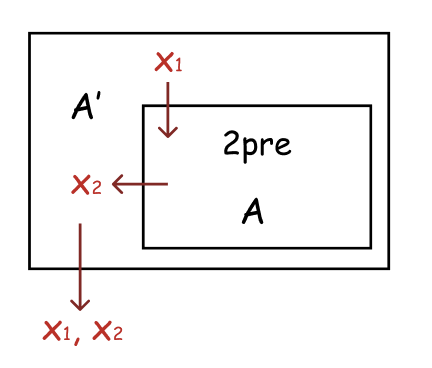
\includegraphics[scale=0.6]{figures/2pre.png}
    \caption{2nd-preimage game visualization: Follows \ref{a'} construction, in which $\mathcal{A}'$ produces $x_1$ and gives $x_1$ to $\mathcal{A}$. Then, $\mathcal{A}$ provides $x_2$ and $\mathcal{A}'$ returns $x_1, x_2$.}
    \label{fig:2pre_viz}
\end{figure}

\end{proof}

\begin{theorem}
% Hash $H$ has $\mathsf{2PRE}_\mathcal{A}$ security $\implies$ $H$ has $\mathsf{PRE}_\mathcal{A}$ security.
If $H$ is 2nd-preimage resistant, then $H$ is preimage resistant.
\end{theorem}

\begin{proof}
For the sake of contradiction, suppose that $H$ is not preimage resistant.  Then, there exists an  adversary against preimage. We construct $\mathcal{A}'$ against 2nd-preimage resistance \ref{a'2}.

\begin{algorithm}[H]
\caption{$\mathcal{A}'$ Construction}
\label{a'2}
\begin{algorithmic}[1]
\Function{$\mathcal{A}'$}{$1^\kappa$}:
    \State $x \leftarrow R \{0,1\}^{2\kappa+1}$
    \State $y \leftarrow H(x)$
    \State $x' \leftarrow \mathcal{A}(y)$
    \State \textbf{return} $x' \ne x_1 \wedge H(x')=H(x)$
\EndFunction
\end{algorithmic}
\end{algorithm}

\begin{figure}[H]
    \centering
    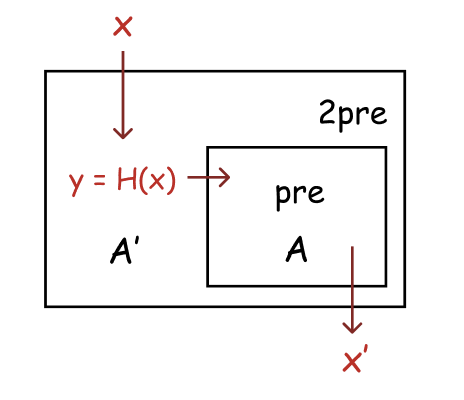
\includegraphics[scale=0.6]{figures/pre.png}
    \caption{Preimage game visualization: Follows \ref{a'2} construction, in which $\mathcal{A}'$ produces $y = H(x)$ given $x$. Then, give $y$ to $\mathcal{A}$ to produce $x'$.}
    \label{fig:pre_viz}
\end{figure}

We hope $x'\ne x$. Partition the input space into "boxes" ($y$: output value) containing dots ($x$: input value) that all hash to the same value. Sort boxes by their sizes (number of inputs) in ascending order, in which the larger boxes are on the left. The purpose of this is that we want to argue that it's harder to guess a dot in a larger box.

Next, we split into two halves of equal number of inputs ($2^{2\kappa}$ dots each half). It is impossible to have $< 2^\kappa$ dots in a "box" on the left half because then each box on the right half has $<2^\kappa$. There are $<2^\kappa$ boxes on the right half, each with $<2^\kappa$ dots, so the total dots in the right half is $<2^\kappa \cdot 2^\kappa = 2^{2\kappa} \implies $ there are $<2^{2\kappa}$ dots.
So, all the left-half boxes are "large".
The probability that we sampled an input on the left half = $\frac{1}{2}$ (sampling uniformly). The $y$ value of the box of our input will have $\geq 2^\kappa$. The adversary has no better strategy than guessing uniformly at random from the box. \\
Thus, there holds: $Pr[\mathsf{2PRE}_\mathcal{A}'(\kappa)] \geq Pr[\mathsf{PRE}_\mathcal{A}(\kappa)=1](\frac{1}{2})(1-2^{-\kappa})$
= non-negligible * constant * value close to 1 = non-negligible. So $Pr[\mathsf{2PRE}_\mathcal{A}'(\kappa)]$ is non-negligible. This implies that $\mathsf{2PRE}$ security is broken, in contradiction.
\end{proof}

\section{Transactions and Signatures}
\textbf{Verifiability of money}: If money is created correctly, money has verifiability property such as ownership validation. Here, we discuss a transfer of ownership.

In blockchain networks, a transaction is an entry in local state. Each node keeps a ledger, which is a recorded sequence of transactions ("tx"s). Ledgers are used to verify and update the system state, a record of the balances of all parties in the system, such that consensus across nodes is maintained.

Assume we have parties $A$, $B$, $C$, etc. Each party can have some sort of money and each party will share all financial information. An example of a transaction could be party $A$ saying "Give 5 units to party $B$." The following is an outline of ledger/transaction procedures:
\begin{enumerate}
    \item
    Initial system state: some distribution of money.
    \item
    Issue a tx by broadcasting
    \item
    Upon receiving a tx:
    \begin{enumerate}
        \item
        Check validity (source has enough money)
        \item
        Append to local ledger
    \end{enumerate}
    \item
    Read ledger to determine balances (system state)
\end{enumerate}

However, nobody should be able to issue transactions spending money from someone's else balance. Therefore, we need to authenticate transactions. One way to achieve it is by using digital signatures.

Digital signature scheme, Alg.~\ref{keys},  consists of three algorithms: key generation, signing and verifying algorithms.
% Key generation algorithms takes a security parameter as an input and outputs a pair of keys - public and private. Signing algorithms takes a message and a private key as an input and outputs a signature for the given message. Verifying algorithms takes as an input a public key, a message and a signature and outputs true if the given signature is valid.
\begin{algorithm}
\caption{Private and Public Keys: Signature Scheme}
\label{keys}
\begin{algorithmic}[1]
    \State $(pk, sk) \leftarrow Gen(1^\kappa)$
    \State $\sigma \leftarrow Sig(sk, m)$
    \State $Ver(pk, m, \sigma) \leftarrow \{\text{True}/\text{False}\}$
\end{algorithmic}
\end{algorithm}

An important property of digital signature scheme is \textbf{correctness}: $\forall m : (pk, sk) \leftarrow Gen(1^{\kappa}) : Ver(pk, m, Sig(sk, m)) = \text{True}$. In other words, for any message, we should be able to verify using a public key and $m$ such that $Ver() = True$. Transactions are happening between public keys and messages are signed with private key by the author, verified by other users via the author's public key. \\

For a signature scheme to be secure, it should be impossible for adversary to produce a valid signature without knowing a private key. More formally,
a security game for digital signatures is defined as follows in Alg~\ref{unforgable}:
\begin{algorithm}
\caption{Signatures are unforgable}
\label{unforgable}
\begin{algorithmic}[1]
\Function{$\mathsf{Forgery}_\mathcal{A}$}{$\kappa$}
    \State $M \leftarrow \emptyset$
    \State $(pk, sk) \leftarrow Gen(1^\kappa)$
    \State $\sigma, m \leftarrow \mathcal{A}^O(pk)$
    \State \textbf{return} $Ver(pk, m, \sigma) \wedge m \notin M$
\EndFunction
\end{algorithmic}
\end{algorithm}

We want to allow the adversary to have access to an oracle such that the adversary can choose an adversarial message. We use $M$ to track the set of messages requested by the adversary. We don't want to allow the adversary to simply invoke the oracle \ref{oracle} function and return a forged messaged outputted by $M$.

\textbf{Oracle}, that can be called by the adversary is defined in Alg.~\ref{oracle}.
\begin{algorithm}
\caption{Signatures are unforgable}
\label{oracle}
\begin{algorithmic}[1]
\Function{O}{$m'$}:
    \State $\sigma' \leftarrow Sig(sk, m')$
    \State $M \leftarrow M \cup \{m'\}$
    \State \textbf{return} $\sigma'$
\EndFunction
\end{algorithmic}
\end{algorithm}
